\documentclass[crop, tikz]{standalone}

\usepackage[utf8]{inputenc}

\usetikzlibrary{calc}

\begin{document}
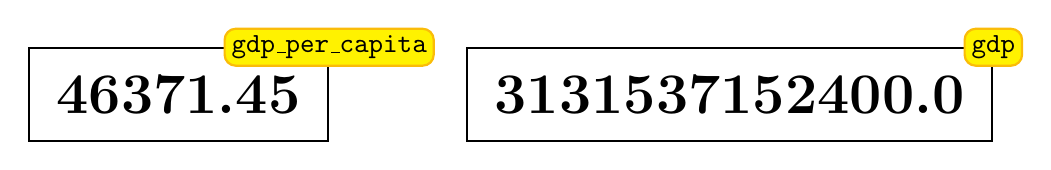
\begin{tikzpicture}[auto,
        label/.style=
            {
                rectangle,
                draw = yellow!50!orange,
                thick,
                fill = yellow,
                inner sep = 0.25em,
                align = center,
                rounded corners
            },
        value/.style=
            {
                rectangle,
                draw = black,
                thick,
                fill = white,
                inner sep = 1em,
                align = center,
                minimum height = 2em
            }
    ]

    \draw (-3.5,0) node[value] (A) {\huge \textbf{46371.45}};
    \draw (A.north east) node[label] {\tt gdp\_per\_capita};

    \draw (3.5,0) node[value] (B) {\huge \textbf{3131537152400.0}};
    \draw (B.north east) node[label] {\tt gdp};

\end{tikzpicture}

\end{document}